\chapter{Implementierung}
Die Umsetzung der zu Beginn beschriebenen Funktionalitäten wird innerhalb der folgenden Teilabschnitte beschrieben. Der erste Teilabschnitt dieses Kapitels dokumentiert die entwickelte Software \cite{badps2}, welche den Mikrocontroller steuert und den Programmablauf der einzelnen Funktionalitäten zeigt. Der zweite Teil dieses Kapitels erläutert den Aufbau der Elektronik und zeigt wie die verwendete Hardware mit dem Mikrocontroller zusammengebaut wurde.



\section{Softwaredokumentation}
Die implementierten Softwarekomponenten \cite{badps2} gliedern sich in die drei  Diese beinhalten Hilfsfunktionen für die Tastatur, für die SD-Karte und für die Webseite, welche vorab in den nächsten Abschnitten beschrieben werden.

\subsection{Hilfsfunktionen für die Tastatur}
\subsubsection{void initKeys(int dataPin, int clockPin)}
\subsubsection{void setHigh(int pin)}
\subsubsection{void setLow(int pin)}
\subsubsection{unsigned char readKeys(int dataPin, int clockPin)}
\subsubsection{void sendKeys(int dataPin, int clockPin, unsigned char data)}
\subsubsection{void writeKeys(unsigned char data)}


\subsection{Hilfsfunktionen für die SD-Karte}
\subsubsection{void initCard(int sdPin)}
\subsubsection{String readFile(char* filename)}
\subsubsection{void writeFile(char* filename, String content)}
\subsubsection{void deleteFile(char* filename)}


\subsection{Hilfsfunktionen für die Webseite}
\subsubsection{void sendWebsite(EthernetClient client, String serverState)}


\subsection{Aufnahme von Tastatureingaben}
\begin{figure}
  \centering
  %\includegraphics[angle=90,width=1\textwidth]{images/diagram_reader.png}
  \caption{Aktivitätsdiagramm für die Methode reader()}
  \label{diagram_reader}
\end{figure}


\subsection{Wiedergabe von Tastatureingaben mittels SD-Karte}
\begin{figure}
  \centering
  %\includegraphics[angle=90,width=1\textwidth]{images/diagram_writer.png}
  \caption{Aktivitätsdiagramm für die Methode writer()}
  \label{diagram_writer}
\end{figure}


\subsection{Wiedergabe von Tastatureingaben über Ethernet}
\begin{figure}
  \centering
  %\includegraphics[angle=90,width=1\textwidth]{images/diagram_sender.png}
  \caption{Aktivitätsdiagramm für die Methode sender()}
  \label{diagram_sender}
\end{figure}


\subsection{Gesamter Programmablauf}



\section{Aufbau der Elektronik}
Verwendete Kabel \cite{ps2male} \cite{ps2female}, Arduino Mega und Ethernet \cite{arduino} und PS/2-Tastatur.
\begin{figure}
  \centering
  \begin{minipage}{0.45\textwidth}
    \centering
    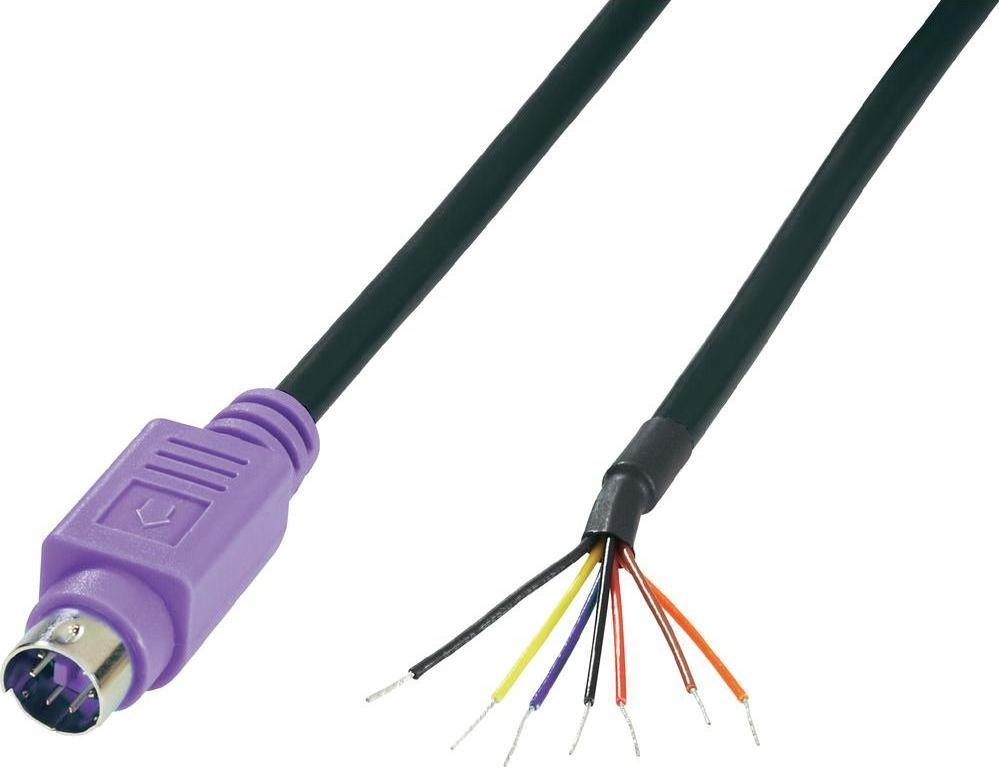
\includegraphics[width=1\textwidth]{images/ps2_male.jpg}
    \caption{PS/2 Male}
    \label{ps2_male}
  \end{minipage}
  \begin{minipage}{0.45\textwidth}
    \centering
    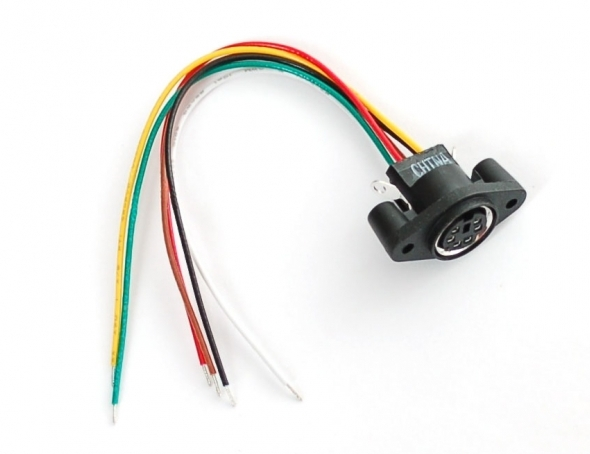
\includegraphics[width=1\textwidth]{images/ps2_female.jpg}
    \caption{PS/2 Female}
    \label{ps2_female}
  \end{minipage}
\end{figure}

\begin{figure}
  \centering
  %\includegraphics[width=0.8\textwidth]{images/hall_effect_sensor.jpg}
  \caption{Schema des Aufbaus fritzing}
  \label{fritzing}
\end{figure}

\begin{figure}
  \centering
  %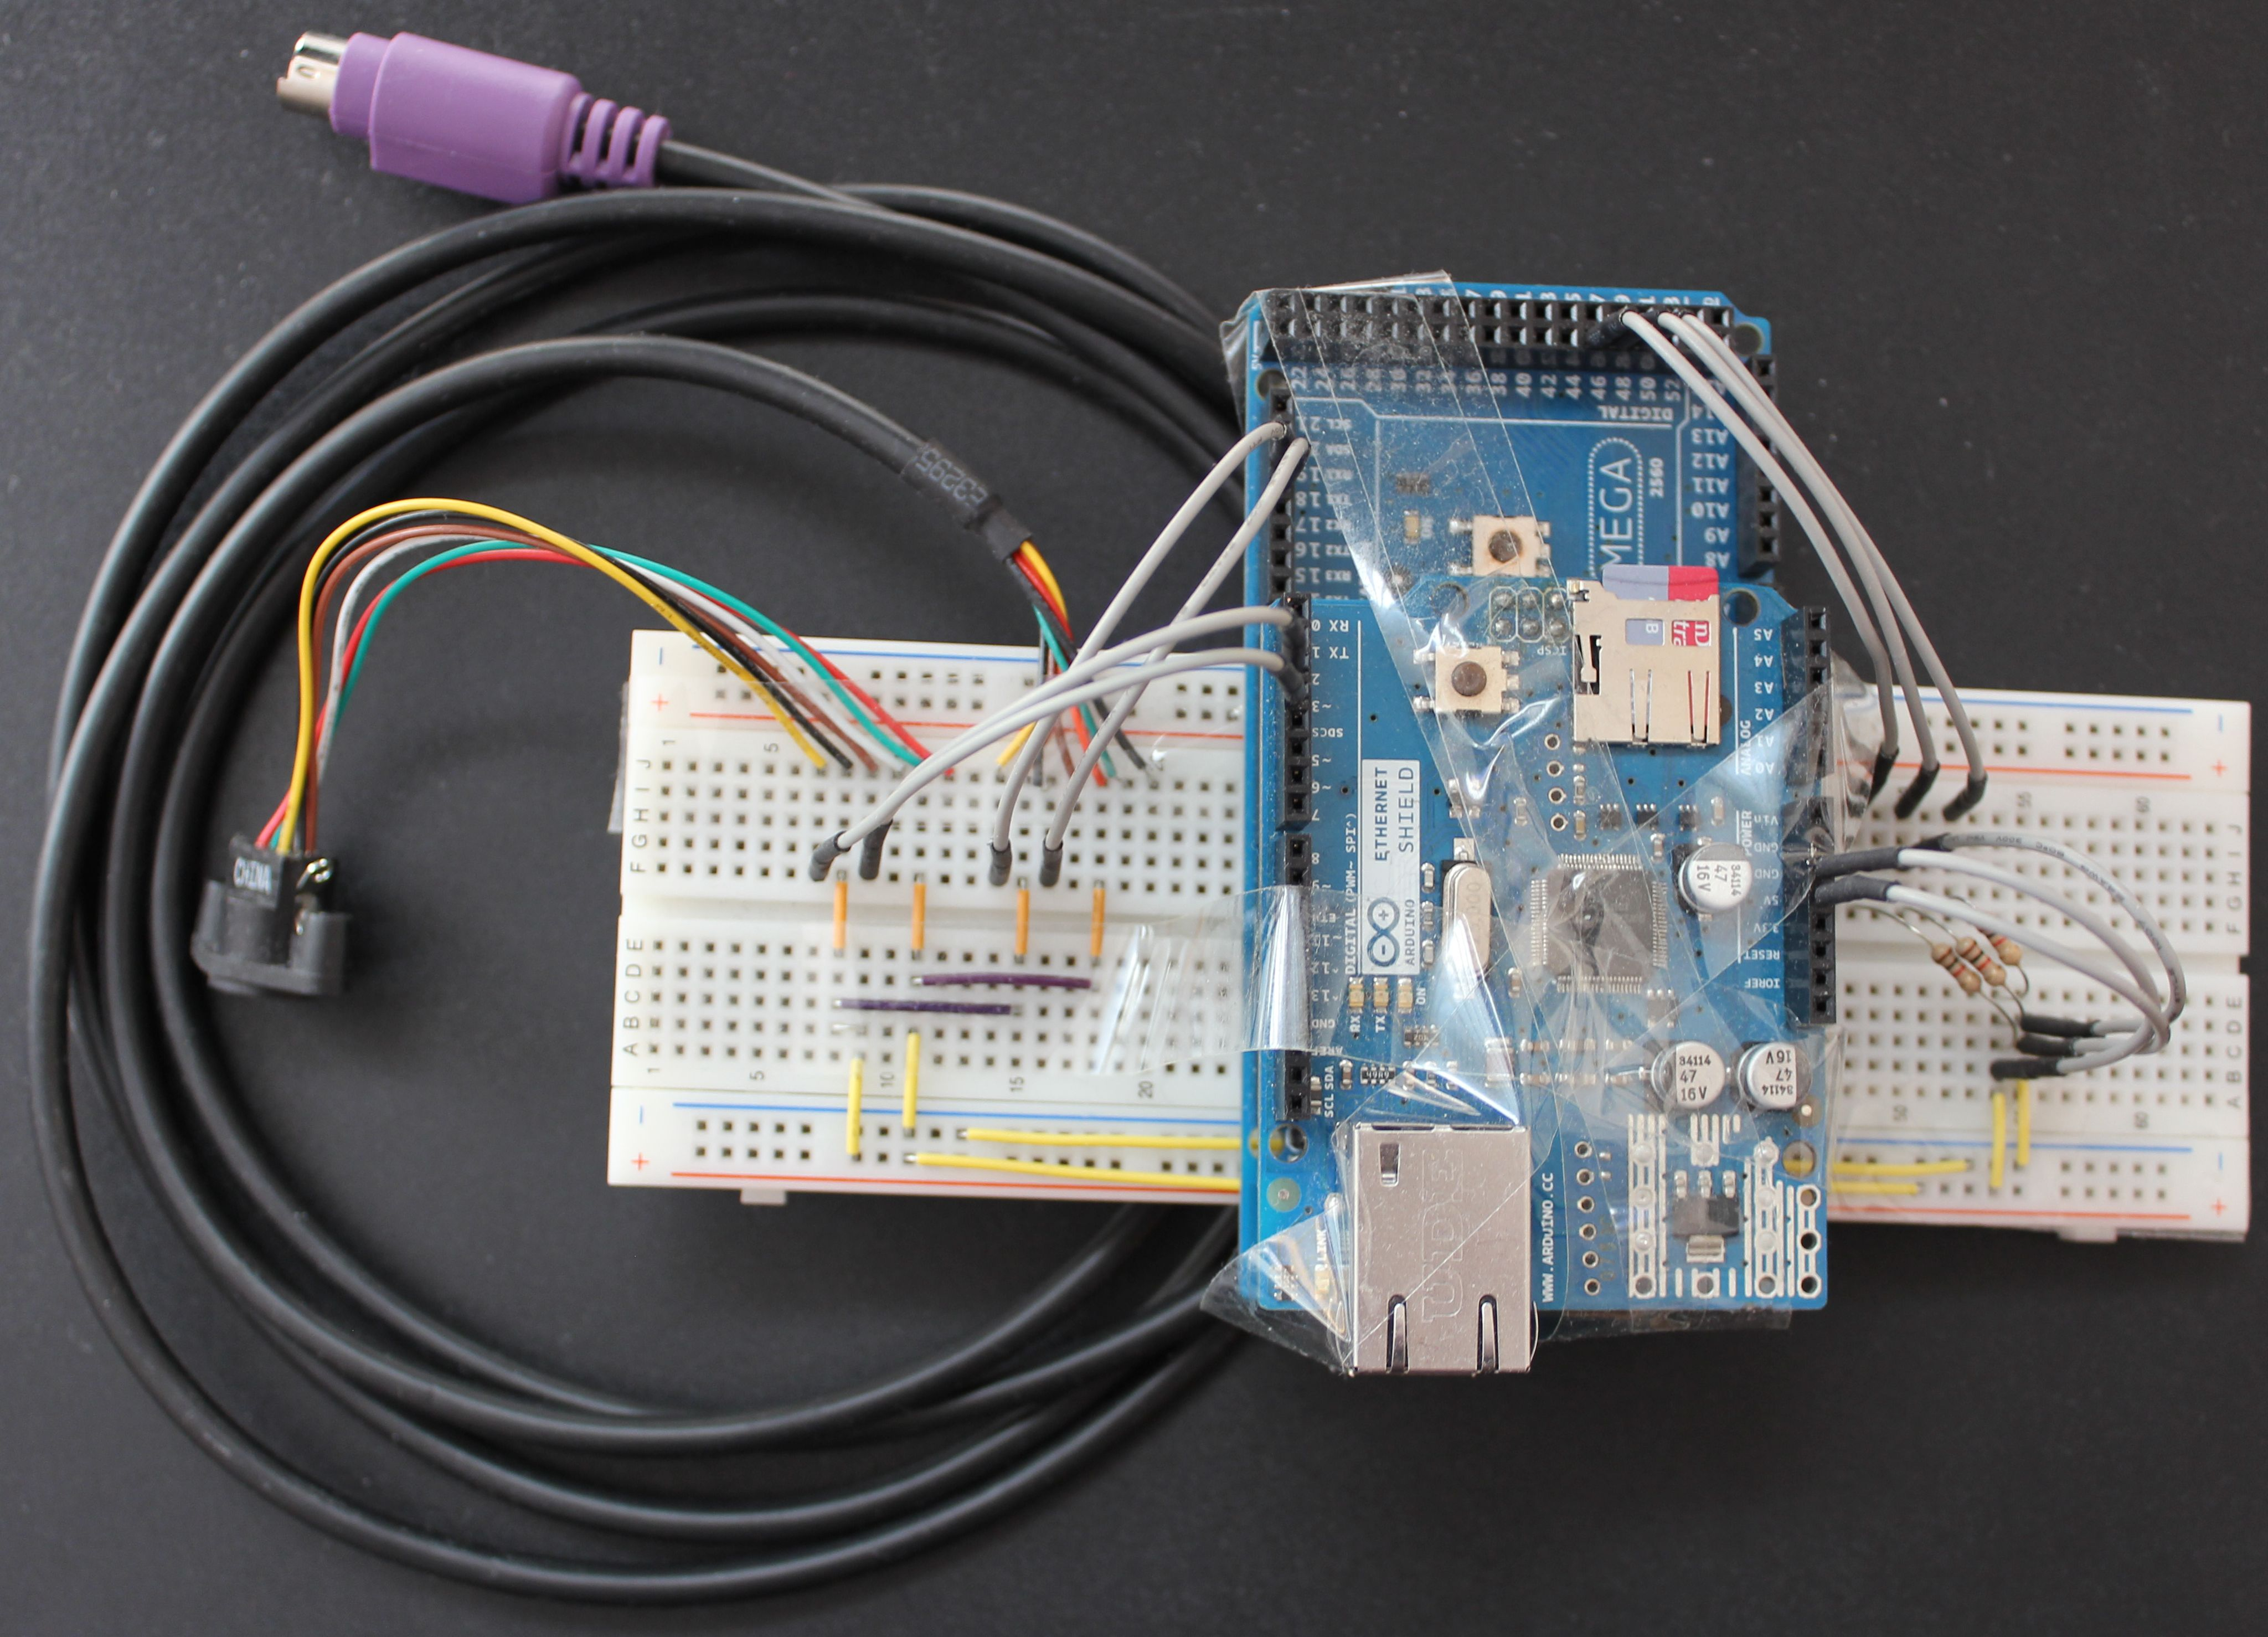
\includegraphics[width=0.8\textwidth]{images/foto1.jpg}
  \caption{Foto des Arduino Ethernet Shields und des Mega 2560 Boards}
  \label{foto1}
\end{figure}